\documentclass[compress]{beamer}

\usetheme{m}

\usepackage{booktabs}

\title{A clean, modern beamer theme}
\subtitle{}
\date{\today}
\author{Matthias Vogelgesang}
\institute{Institute for foo bar}


\begin{document}

\maketitle

\begin{frame}{The mtheme}

  The \emph{mtheme} is a clean beamer theme based on Fira Sans.

  Sections separate frames of the same topic. They also have a nice progress
  indicator.

\end{frame}

\section{Elements}

\begin{frame}{Typography}
  This is with \emph{emphasis} on that sometimes sets \alert{accents} but never
  comes across outright \textbf{bold}. The class style is hosted at
  \url{http://github.com/matze/mtheme}.

  How much space do we need?
\end{frame}

\begin{frame}{Lists}
  \begin{itemize}
    \item Milk
    \item Eggs
    \item Potatos
  \end{itemize}

  \begin{enumerate}
    \item First,
    \item Second and
    \item Last.
  \end{enumerate}

  \begin{description}
    \item[PowerPoint] Meeh.
    \item[Beamer] Yeeeha.
  \end{description}
\end{frame}

\begin{frame}{Animation}
  \begin{itemize}[<+- | alert@+>]
    \item \alert<4>{Hey}
    \item Ho
    \item Let's go
  \end{itemize}
\end{frame}

\begin{frame}{Figures}
  Figures play a vital role to \emph{visualize} an idea. Here's one made with
  TikZ:

  \begin{figure}
    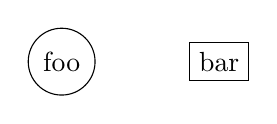
\begin{tikzpicture}
      \node[circle, draw=black] at (0, 0) {foo};
      \node[rectangle, draw=black] at (2, 0) {bar};
    \end{tikzpicture}
    \caption{A circle and a rectangle.}
  \end{figure}
\end{frame}

\begin{frame}{Tables}
  \begin{table}
    \caption{A table}
    \begin{tabular}{lll}
      \toprule
      Foo & Bar & Baz\\
      \midrule
      Foo & Bar & Baz\\
      \bottomrule
    \end{tabular}
  \end{table}
\end{frame}

\begin{frame}{Blocks}

  \begin{block}{A descriptive title}
    Blocks can give your slides structure. Unfortunately, most themes put fling
    them right at your face.
  \end{block}

  Maybe we should play outside.

\end{frame}

\begin{frame}{Math}
  \begin{equation*}
    I_c(x,y) = \sum_{i=-n}^n\sum_{j=-n}^n w\left(
      \mathcal{N}_{x,y},\ \mathcal{N}_{x-i, y-j}\right)
      \cdot
      I_r(x-i,y-j)
  \end{equation*}
\end{frame}

\begin{frame}{Quotes}
  \begin{quote}
    Veni, Vidi, Vici
  \end{quote}
\end{frame}

\section{Conclusion}

\begin{frame}{Summary}
  Get it at

  \begin{center}\url{github.com/matze/mtheme}\end{center}

  or read some non-fiction at

  \begin{center}\url{bloerg.net}\end{center}

  Oh, it's licensed \textsc{cc-by-sa} but you don't need to slap my name on every slide.
\end{frame}

\statement{Questions?}

\end{document}
